% 2006 湖南文科候选卷 Q10；按固定源图的阴影边界重绘，坐标不表示长度比例。
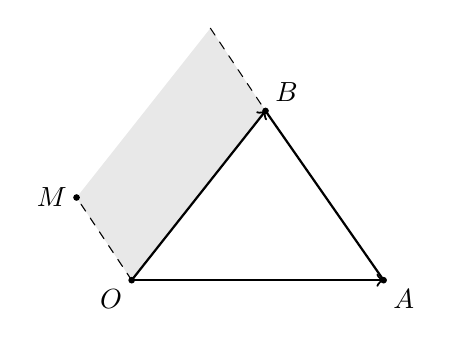
\begin{tikzpicture}[line cap=round,line join=round]
  \coordinate (O) at (0,0);
  \coordinate (A) at (3.2,0);
  \coordinate (B) at (1.7,2.15);
  \coordinate (M) at (-0.7,1.05);
  \coordinate (T) at (1.0,3.2);

  \fill[gray!18] (O)--(M)--(T)--(B)--cycle;

  \draw[dashed] (O)--(M);
  \draw[dashed] (T)--(B);
  \draw[thick] (B)--(A);
  \draw[->,thick] (O)--(B);
  \draw[->,thick] (O)--(A);

  \fill (O) circle[radius=1.2pt];
  \fill (A) circle[radius=1.2pt];
  \fill (B) circle[radius=1.2pt];
  \fill (M) circle[radius=1.2pt];
  \node[below left] at (O) {$O$};
  \node[below right] at (A) {$A$};
  \node[above right] at (B) {$B$};
  \node[left] at (M) {$M$};
\end{tikzpicture}
